\section{Tropical Rainforest}

Tropical rainforests climates or equatorial climates are characterised by frequent and heavy rainfall and are situated on or close to the equator. Because of there locality on earth there are no seasons and therefore very little temperature and illumination variance throughout the year.\\

\subsection{Resource Configuration}

Toamasina, a city in Madagascar at latitude 18\textdegree south, is the location on which climate data is based for these tests.\\

To model a loamy soil, which is common in tropical forests due to its water absorption capabilities, the soil infiltration rate is set to fifteen millimetres per hour (see figure \ref{tab:soil_types}). To model rocky cliff faces, the soil infiltration rate is set to zero when the slope angle surpasses forty degrees.\\

The configured monthly rainfall and rainfall intensity is summarized in figure \ref{fig:results_tropical_input}.\\

The temperature extremes configured are twenty-one degrees for June and twenty-six degrees for December, resulting in monthly temperatures outlined in figure \ref{fig:results_tropical_input}.\\

\begin{figure}
\center
	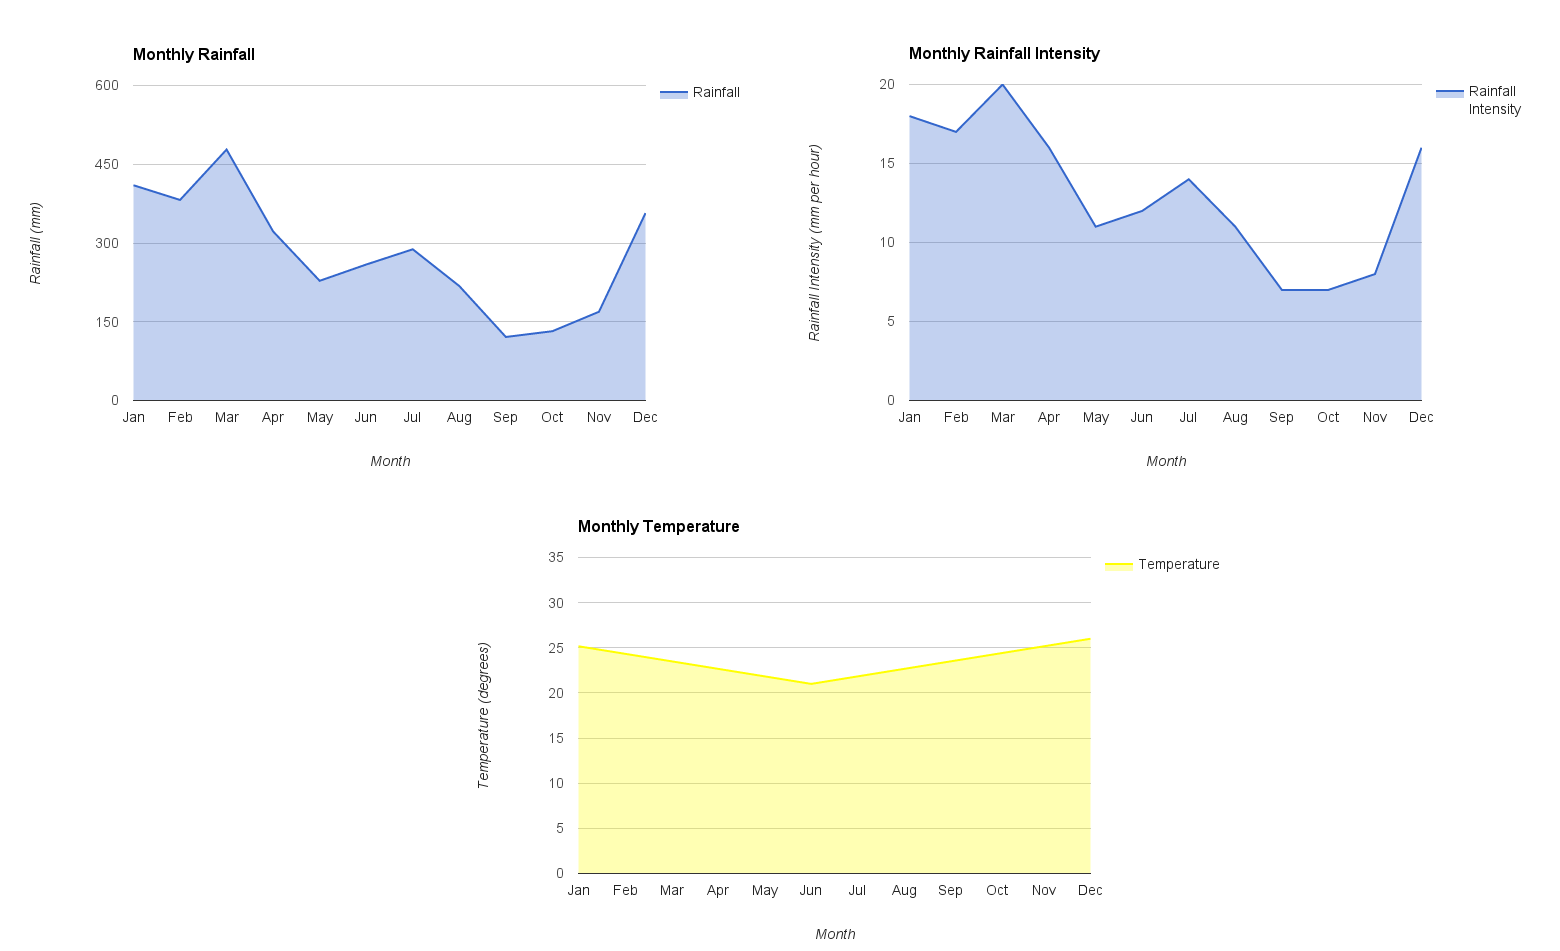
\includegraphics[width=\textwidth]{results_tropical_input.png}
	\caption{ Tropical rainforest: Input resource configurations: Rainfall (top-left), rainfall intensity (top-right) and temperature (bottom).}
	\label{fig:results_tropical_input}
\end{figure}

\subsection{Water Networks}

Given the varying monthly rainfall quantity and intensity, the resulting water networks differ for each month. Figure \ref{fig:results_tropical_water_networks} shows the water networks that form for every month of the year.

\begin{figure}
\center
	\includegraphics[width=\textwidth]{results_tropical_water_networks.png}
	\caption{ Tropical rainforest: Water networks that form on the terrain at every month. From left to right, top to bottom.}
	\label{fig:results_tropical_water_networks}
\end{figure}

\subsection{Clusters}

The number of clusters to generate is set to ten. The clustered terrain is shown in figure \ref{fig:results_tropical_terrain_clusters} and the corresponding cluster properties summarized in figure \ref{fig:results_tropical_cluster_hum_temp_illum} and table \ref{tab:results_tropical_cluster_slope_covarea}. 

\begin{figure}
\center
	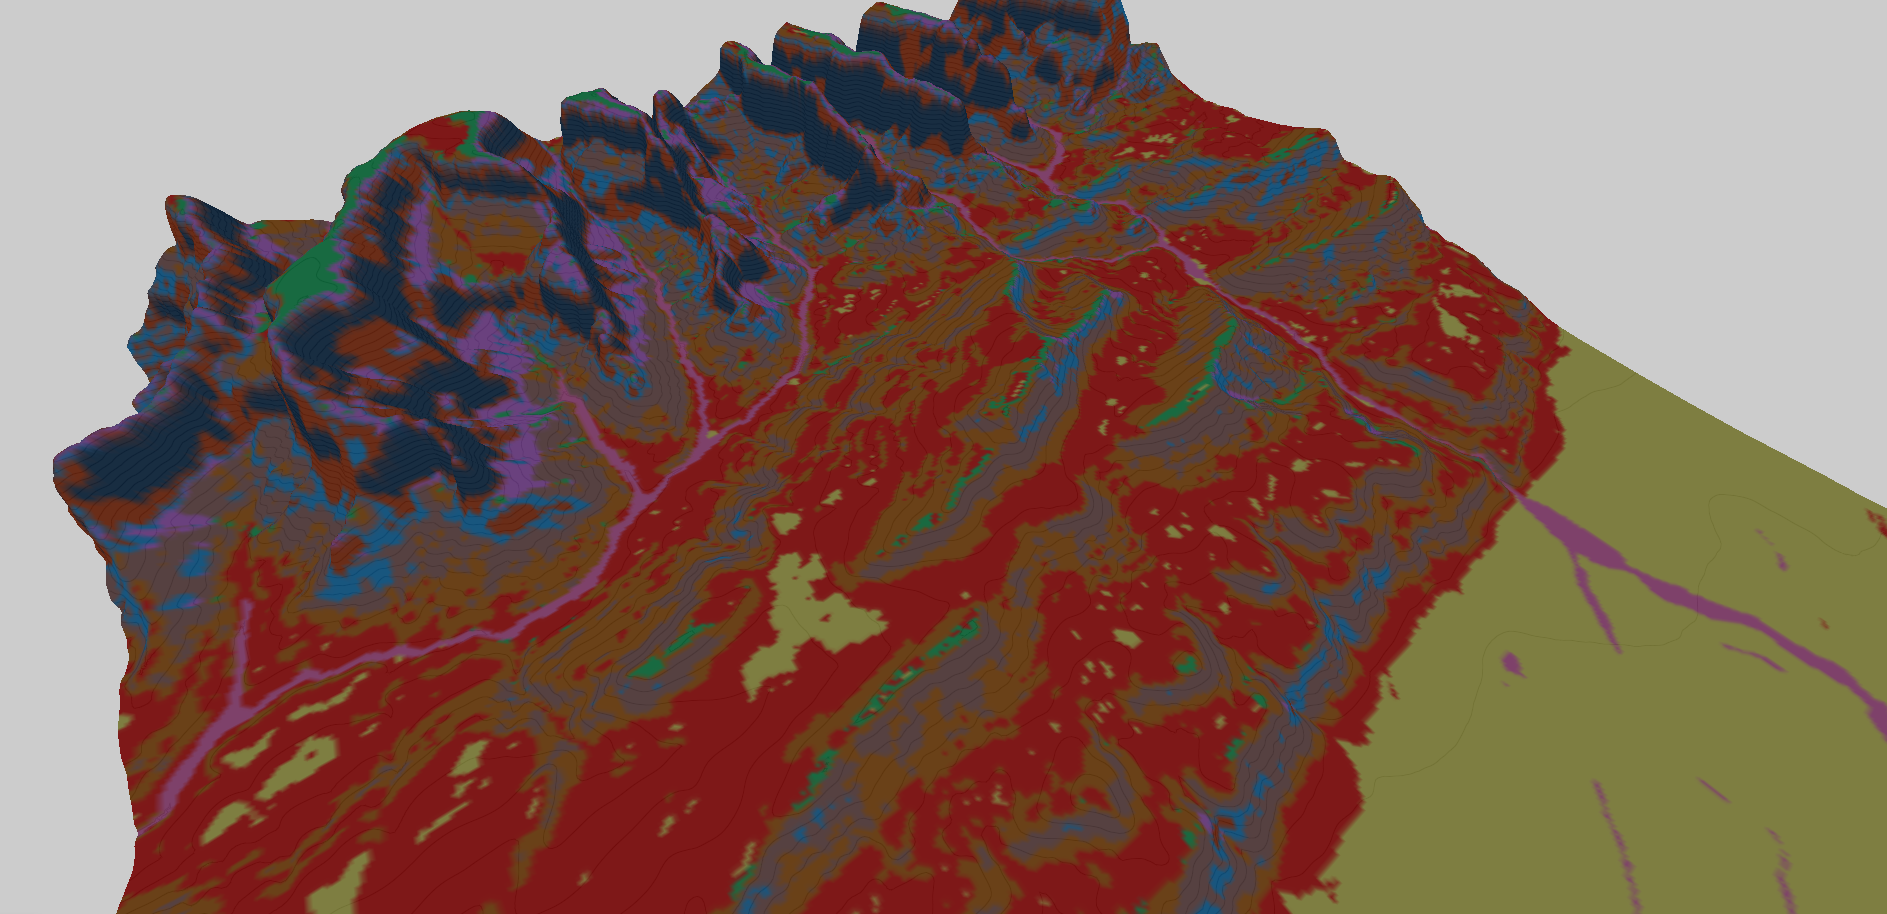
\includegraphics[width=\textwidth]{results_tropical_clusters_on_terrain.png}
	\caption{ Tropical rainforest: Resulting terrain clusters. Refer to table \ref{tab:results_tropical_cluster_slope_covarea} for cluster ID to cluster colour relationships.}
	\label{fig:results_tropical_terrain_clusters}
\end{figure}

\begin{figure}
\center
	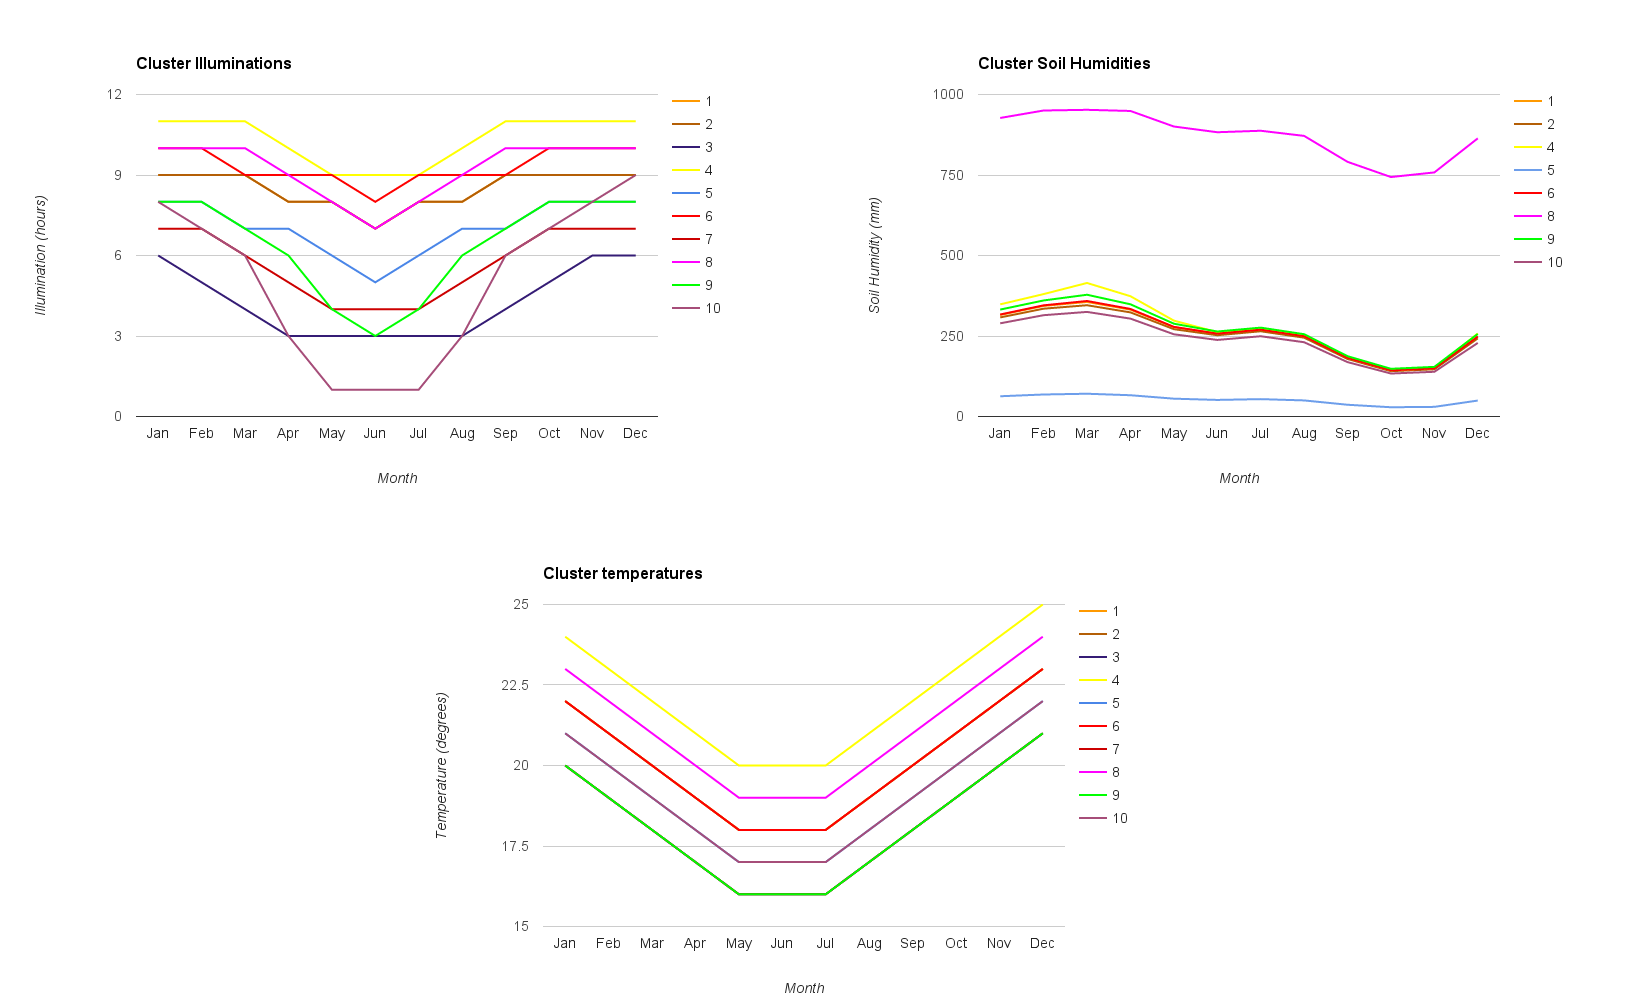
\includegraphics[width=\textwidth]{results_tropical_clusters_hum_temp_illum.png}
	\caption{ Tropical rainforest: Cluster illuminations (top-left). soil humidities (top-right) and temperatures (bottom) for each terrain cluster with color coding to match that of the cluster overlay in figure \ref{fig:results_tropical_terrain_clusters}. Note that soil humidity data is removed for clusters (3 and 7) as the corresponding values are too small.}
	\label{fig:results_tropical_cluster_hum_temp_illum}
\end{figure}

\definecolor{trop_cluster_1}{rgb}{0.8,0.4,0.0}
\definecolor{trop_cluster_2}{rgb}{0.6,0.4,0.4}
\definecolor{trop_cluster_3}{rgb}{0.0,0.2,0.4}
\definecolor{trop_cluster_4}{rgb}{1.0,1.0,0.4}
\definecolor{trop_cluster_5}{rgb}{0.0,0.6,1.0}
\definecolor{trop_cluster_6}{rgb}{1.0,0.0,0.0}
\definecolor{trop_cluster_7}{rgb}{0.8,0.2,0.0}
\definecolor{trop_cluster_8}{rgb}{1.0,0.4,0.8}
\definecolor{trop_cluster_9}{rgb}{0.0,0.8,0.4}
\definecolor{trop_cluster_10}{rgb}{0.8,0.4,1.0}

\begin{table}[h]
  \centering
	    \begin{tabular}{|p{5cm}|p{5cm}|p{5cm}|}
		\hline	
  	    \textbf{Cluster ID} & \textbf{Slope (degrees)} & \textbf{Coverage area (\% of terrain)} \\
  	    \hline	
		\cellcolor{trop_cluster_1} 1 & 22.3 & 19.3 \\
		\hline
		\cellcolor{trop_cluster_2} 2 & 32.2704 & 16.2 \\
		\hline
		\cellcolor{trop_cluster_3} 3 & 69.092 & 4.7 \\
		\hline
		\cellcolor{trop_cluster_4}4 & 2.95581 & 18.1 \\
		\hline
		\cellcolor{trop_cluster_5} 5 & 42.9369 & 4.8 \\
		\hline
		\cellcolor{trop_cluster_6} 6 & 11.8319 & 22.1 \\
		\hline
		\cellcolor{trop_cluster_7} 7 & 54.1674 & 6.0 \\
		\hline
		\cellcolor{trop_cluster_8} 8 & 8.0803 & 2.1 \\
		\hline
		\cellcolor{trop_cluster_9} 9 & 14.0102 & 2.5 \\
		\hline
		\cellcolor{trop_cluster_10} 10 & 32.1679 & 3.8 \\
		\hline
		\end{tabular}
		\caption{Tropical rainforest: Cluster slope and coverage area with color coding matching the cluster overlay in figure \ref{fig:results_tropical_terrain_clusters}.}
	  \label{tab:results_tropical_cluster_slope_covarea}
\end{table}

\subsection{Vegetation}

Five tropical rainforest plant species are configured for this test: \textit{Brazil nut}, \textit{Cavendish banana}, \textit{Heliconia}, \textit{King of Bromeliads} and \textit{Orchid}. The properties associated with each are summarized in appendix \ref{AppendixE}.\\

The specie suitability filtering (see section \ref{sec:plant_suitability_filtering}) automatically filters out some species from being inserted in some clusters as the resources of the given clusters did not meet the requirements of the given species. Table \ref{tab:results_tropical_species_suitability} summarizes this information and illustrates the species which are suited to individual clusters and, if not, the resource which prevents it. From this, it is possible to conclude that no plants are able to grow, and therefore no ecosystem simulator needs to be run, for clusters 3, 5, 7 and 8. \textit{Clusters 3, 5 and 7} have to steep a slope and too little soil humidity to cater for these species. \textit{Cluster 8} has too moist soil as it represents the points on the terrain with standing water.\\

\definecolor{color_red}{rgb}{1.0,0.0,0.0}
\definecolor{color_green}{rgb}{0.0,1.0,0.0}
\definecolor{color_orange}{rgb}{1.0,0.65,0.0}

\begin{table}[h]
  \centering
	    \begin{tabular}{|p{2cm}|p{2.5cm}|p{2.5cm}|p{2.5cm}|p{2.5cm}|p{2.5cm}|}
		\hline	
		&  \textbf{Orchid} & \textbf{Cavendish banana} & \textbf{Heliconia} & \textbf{Brazil Nut} & \textbf{King of Bromeliads}\\
		\hline	
		Cluster 1 & 
		Y & 
		Y & 
		Y & 
		Y & 
		Y \\
		\hline	
		Cluster 2 & 
		Y & 
		\cellcolor{color_red}N (S$^{+}$) & 
		Y & 
		\cellcolor{color_red}N (S$^{+}$) & 
		Y \\
		\hline	
		Cluster 3 & 
		\cellcolor{color_red}N (S$^{+}$, SH$^{-}$) & 
		\cellcolor{color_red}N (S$^{+}$, SH$^{-}$) & 
		\cellcolor{color_red}N (S$^{+}$, SH$^{-}$) & 
		\cellcolor{color_red}N (S$^{-}$, SH$^{-}$) & 
		\cellcolor{color_red}N (S$^{+}$, SH$^{+}$) \\
		\hline	
		Cluster 4 & 
		Y & 
		Y & 
		Y & 
		Y & 
		Y \\
		\hline	
		Cluster 5 & 
		\cellcolor{color_red}N (SH$^{-}$) & 
		\cellcolor{color_red}N (S$^{+}$, SH$^{-}$) & 
		\cellcolor{color_red}N (S$^{+}$, SH$^{-}$) & 
		\cellcolor{color_red}N (S$^{+}$, SH$^{-}$) & 
		\cellcolor{color_red}N (SH$^{-}$) \\
		\hline	
		Cluster 6 & 
		Y & 
		Y & 
		Y & 
		Y &
		Y \\
		\hline	
		Cluster 7 & 
		\cellcolor{color_red}N (SH$^{-}$) &
		\cellcolor{color_red}N (S$^{+}$, SH$^{-}$) &
		\cellcolor{color_red}N (S$^{+}$, SH$^{-}$) & 
		\cellcolor{color_red}N (S$^{+}$, SH$^{-}$) & 
		\cellcolor{color_red}N (S$^{+}$, SH$^{-}$) \\
		\hline	
		Cluster 8 & 
		\cellcolor{color_red}N(SH$^{+}$) & 
		\cellcolor{color_red}N (SH$^{+}$) & 
		\cellcolor{color_red}N (SH$^{+}$) & 
		\cellcolor{color_red}N (SH$^{+}$) & 
		\cellcolor{color_red}N (SH$^{+}$) \\
		\hline	
		Cluster 9 & 
		Y & 
		Y & 
		Y & 
		Y & 
		Y \\
		\hline	
		Cluster 10 &
		Y & 
		\cellcolor{color_red}N (S$^{+}$) & 
		Y & 
		\cellcolor{color_red}N (S$^{+}$) & 
		Y \\
		\hline	
		\end{tabular}
		\caption{Tropical rainforest: Summary of species suitability to each cluster. When a species is not suited, the reason is stated in brackets where \textit{S} is the slope, \textit{SH} is the soil humidity, $^{+}$ signifies too much and $^{-}$ too little of the given resource.}
	  \label{tab:results_tropical_species_suitability}
\end{table}

Figures \ref{fig:results_tropical_brazil_nut_suitability}, \ref{fig:results_tropical_cavendish_banana_suitability}, \ref{fig:results_tropical_heliconia_suitability}, \ref{fig:results_tropical_king_of_bromeliads_suitability}, \ref{fig:results_tropical_orchid_suitability} and table \ref{tab:results_tropical_species_slope_suitability} illustrate how suited the remaining clusters are for each plant species. From this, it is possible to conclude that: \textit{Clusters 9 and 10} prevents \textit{Brazil Nut}, \textit{Cavendish Banana} and \textit{Heliconia} from growing as their minimum illuminations goes below these species lower limits. These clusters also prevents shade-loving \textit{King of Bromeliads} and \textit{Orchids} from growing as their maximum illuminations surpasses the species upper limits. Clusters 9 and 10 are therefore unsuited to all species and, therefore, an empty distribution should be output from the ecosystem simulator for these clusters.\\
\textit{Cavendish Banana} and \textit{Brazil Nut} plants are unsuited to clusters 1 and 2 as the clusters minimum illumination goes below the species lower limit.\\
\textit{King of Bromeliads} and \textit{Orchids} are unsuited to all clusters as their maximum illuminations surpass the species upper-limit. However, as these species are shade-loving, there is a possibility they survive in the undergrowth of striving plant instances.\\
Given all this, the clusters in which plant species are suited and a plausible distributions created are clusters 1, 2, 4 and 6. Together, these clusters make up 70\% of the terrain.\\

\begin{figure}
\center
	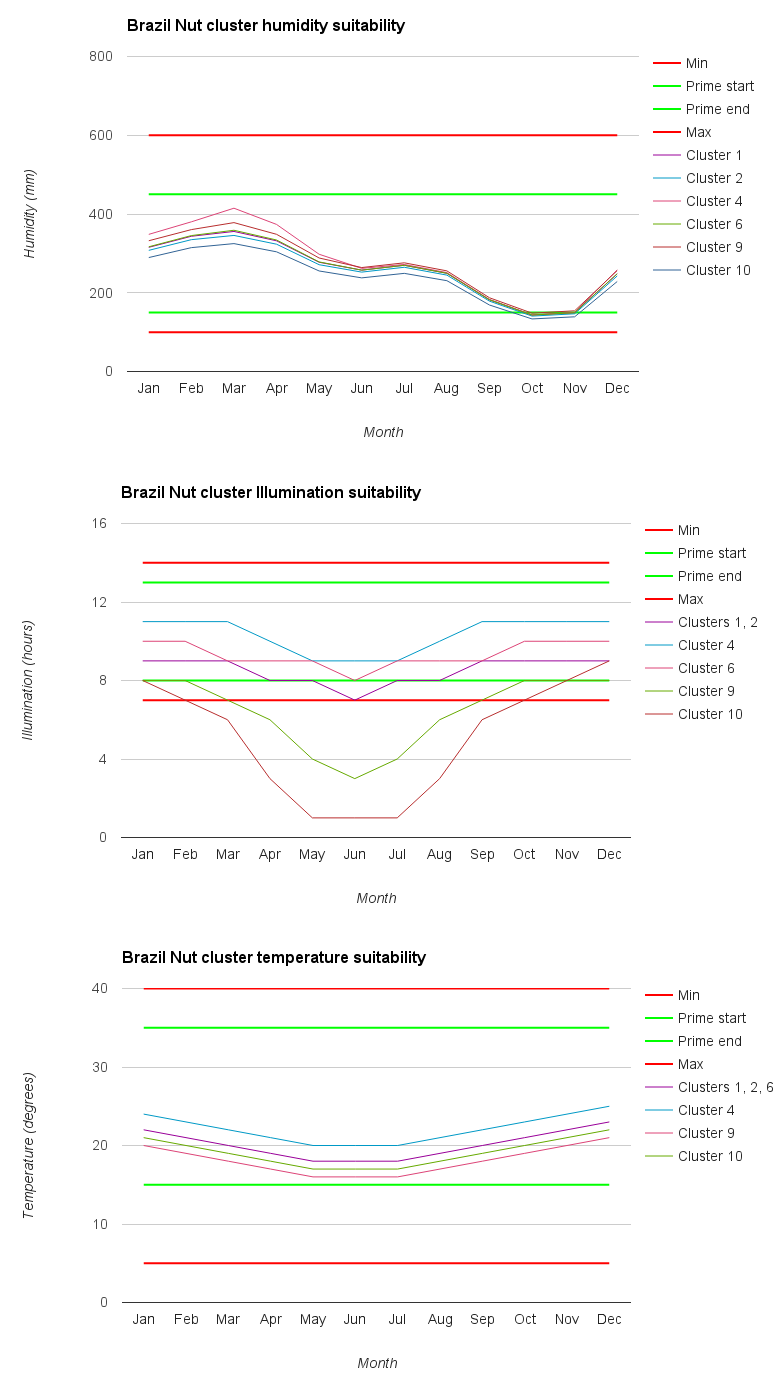
\includegraphics[width=\textwidth]{brazil_nut_suitability.png}
	\caption{ Tropical rainforest: Brazil nut suitability to clusters 1, 2, 4, 6, 9 and 10 in terms of temperature (top-left), illumination (top-right) and soil humidity (bottom). The thick green lines and red lines delimit the species prime range and absolute limits respectively. Note that the illuminations are identical for clusters 1 and 2 and the temperatures are identical for clusters 1, 2 and 6. }
	\label{fig:results_tropical_brazil_nut_suitability}
\end{figure}

\begin{figure}
\center
	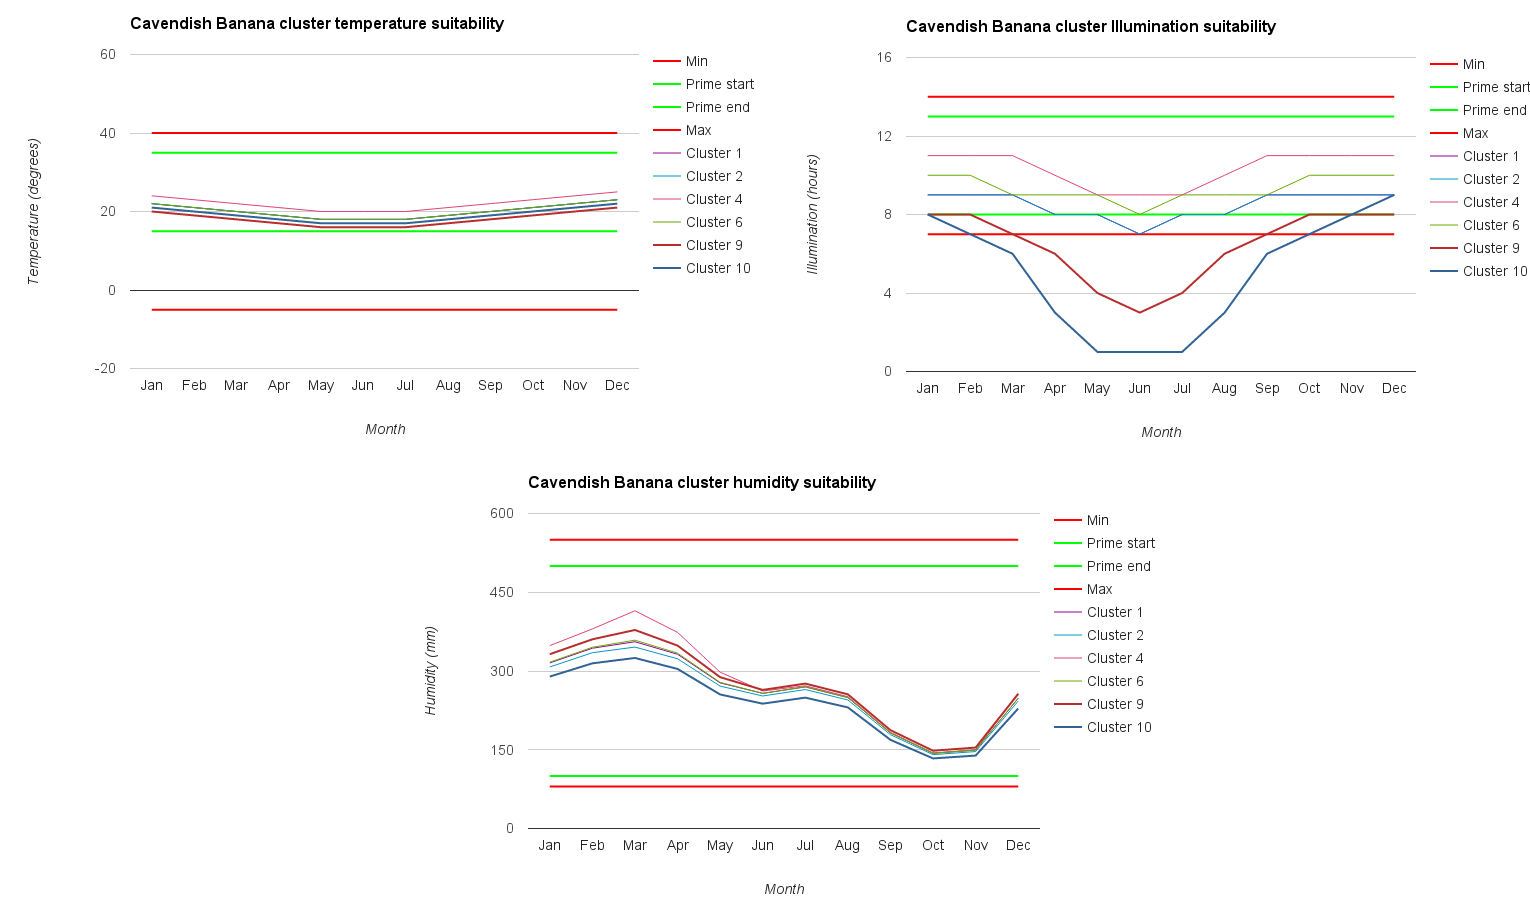
\includegraphics[width=\textwidth]{cavendish_banana_suitability.png}
	\caption{ Tropical rainforest: Cavendish Banana suitability to clusters 1, 2, 4, 6, 9 and 10 in terms of temperature (top-left), illumination (top-right) and soil humidity (bottom). The thick green lines and red lines delimit the species prime range and absolute limits respectively. Note that the illuminations are identical for clusters 1 and 2 and the temperatures are identical for clusters 1, 2 and 6.}
	\label{fig:results_tropical_cavendish_banana_suitability}
\end{figure}

\begin{figure}
\center
	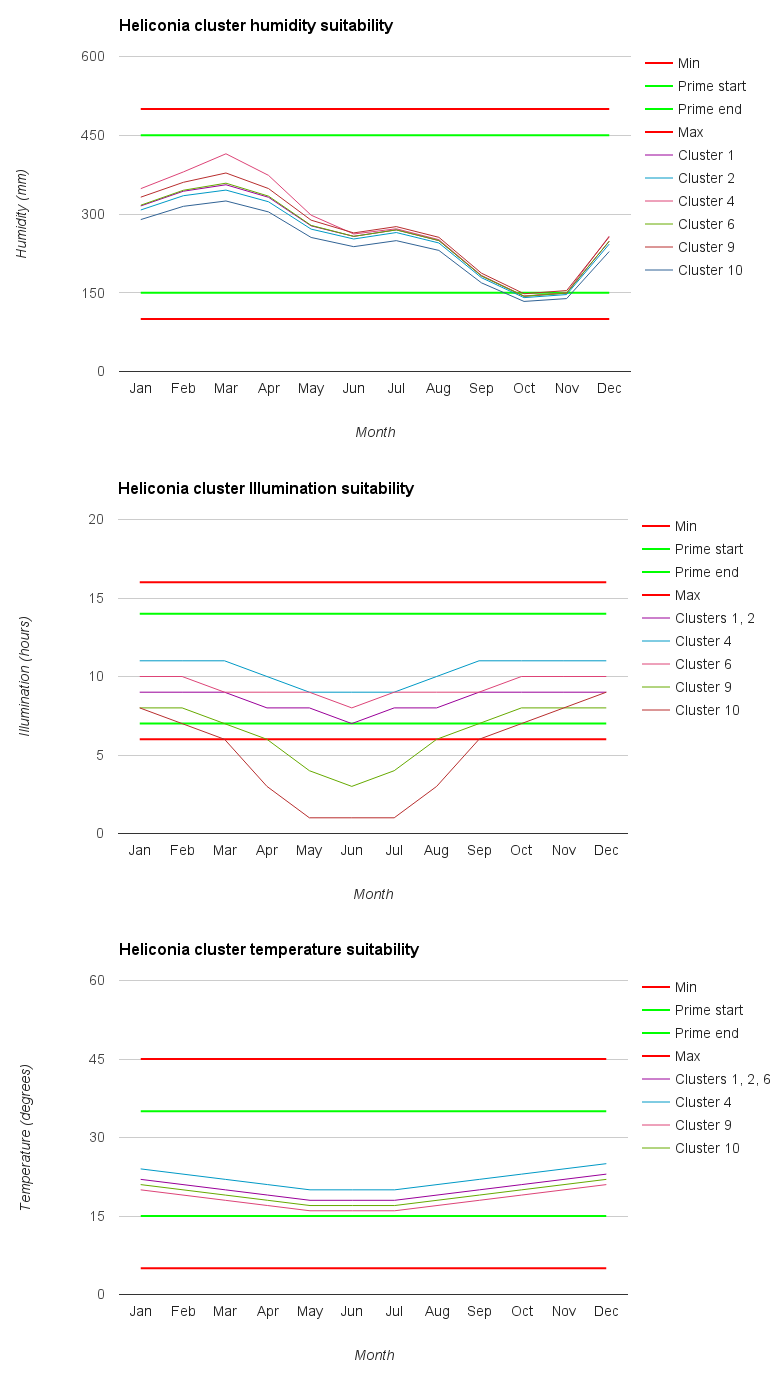
\includegraphics[width=\textwidth]{heliconia_suitability.png}
	\caption{ Tropical rainforest: Heliconia suitability to clusters 1, 2, 4, 6, 9 and 10 in terms of temperature (top-left), illumination (top-right) and soil humidity (bottom). The thick green lines and red lines delimit the species prime range and absolute limits respectively. Note that the illuminations are identical for clusters 1 and 2 and the temperatures are identical for clusters 1, 2 and 6.}
	\label{fig:results_tropical_heliconia_suitability}
\end{figure}

\begin{figure}
\center
	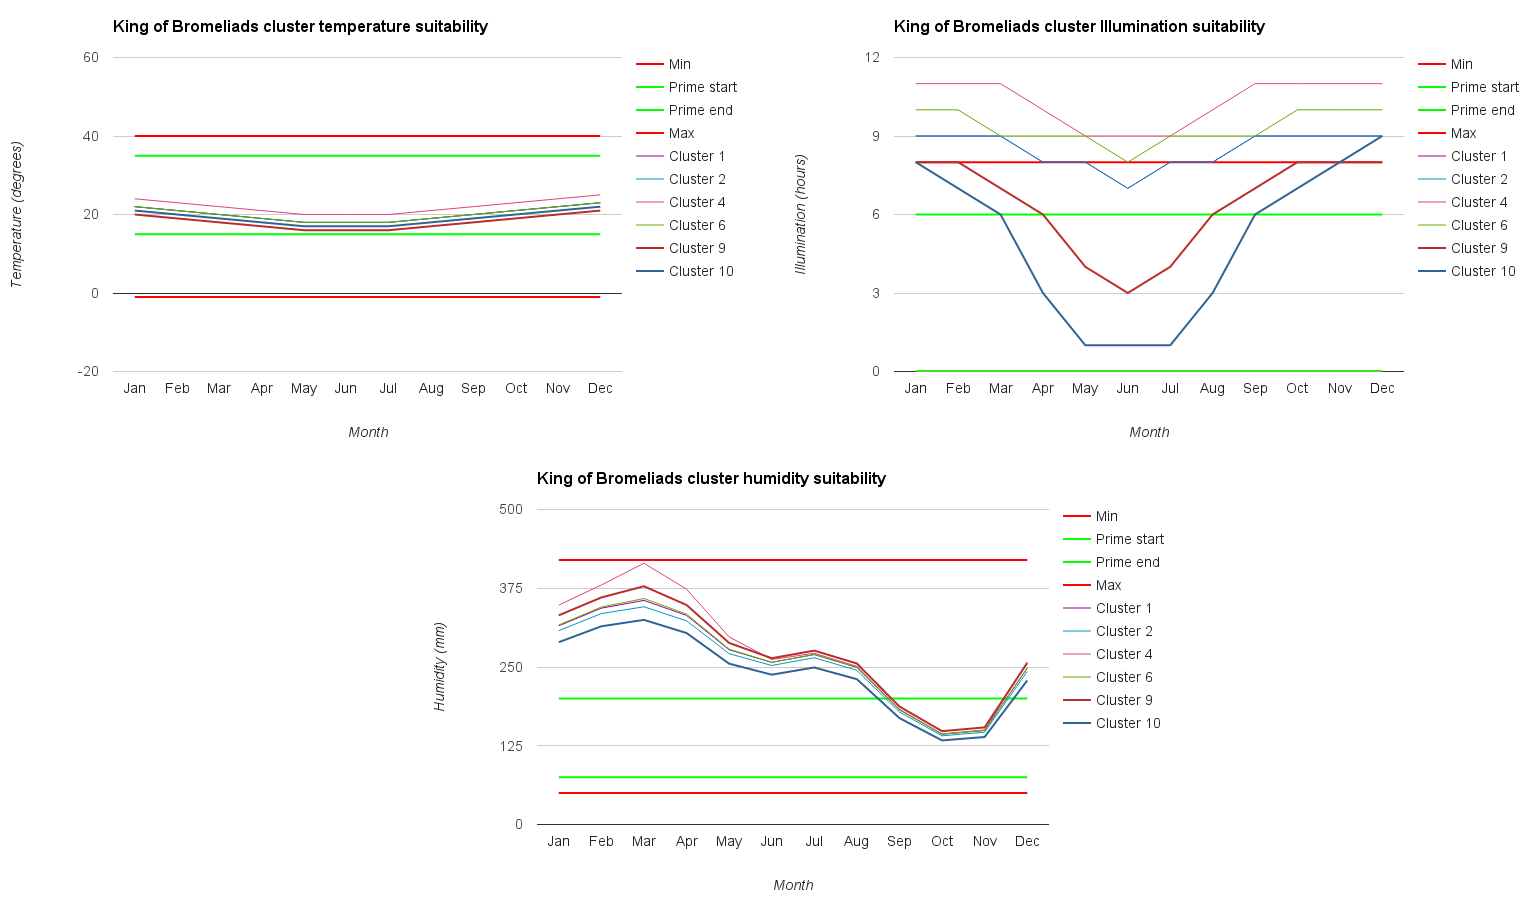
\includegraphics[width=\textwidth]{king_of_bromeliads_suitability.png}
	\caption{ Tropical rainforest: King of Bromeliads suitability to clusters 1, 2, 4, 6, 9 and 10 in terms of temperature (top-left), illumination (top-right) and soil humidity (bottom). The thick green lines and red lines delimit the species prime range and absolute limits respectively. Note that because the king of bromeliads is a shade-loving specie, the minimum illumination line is not present as it is overlapped by the start of prime range line. Note also that the illuminations are identical for clusters 1 and 2 and the temperatures are identical for clusters 1, 2 and 6.}
	\label{fig:results_tropical_king_of_bromeliads_suitability}
\end{figure}

\begin{figure}
\center
	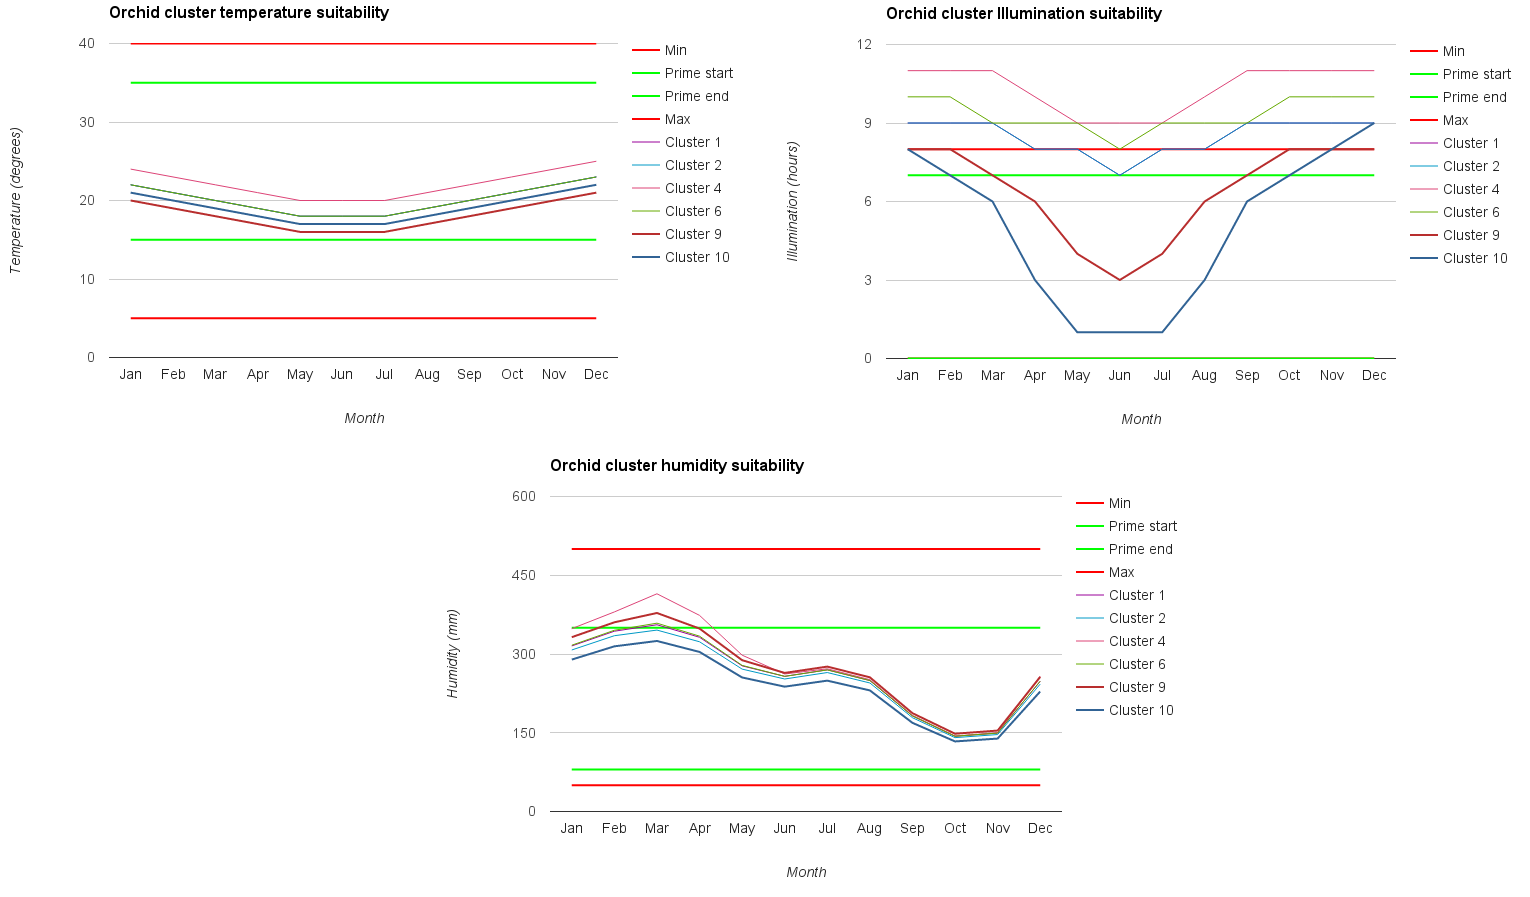
\includegraphics[width=\textwidth]{orchid_suitability.png}
	\caption{ Tropical rainforest: Orchid suitability to clusters 1, 2, 4, 6, 9 and 10 in terms of temperature (top-left), illumination (top-right) and soil humidity (bottom). The thick green lines and red lines delimit the species prime range and absolute limits respectively. Note that because the king of bromeliads is a shade-loving specie, the minimum illumination line is not present as it is overlapped by the start of prime range line. Note also that the illuminations are identical for clusters 1 and 2 and the temperatures are identical for clusters 1, 2 and 6.}
	\label{fig:results_tropical_orchid_suitability}
\end{figure}

\begin{table}[h]
  \centering
	    \begin{tabular}{|p{2cm}|p{2.5cm}|p{2.5cm}|p{2.5cm}|p{2.5cm}|p{2.5cm}|}
		\hline	
  	     & \textbf{Brazil Nut} & \textbf{Cavendish Banana} & \textbf{Heliconia} & \textbf{King of Bromeliads} & \textbf{Orchid} \\
  	    \hline	
		\textbf{Start of decline} & 
		15 & 
		20 & 
		25 &
		35 & 
		35 \\
		\hline
		\textbf{Max} & 
		25 &
		30 &
		40 &
		45 & 
		55 \\
		\hline
		\textbf{Cluster 1} & 
		\cellcolor{color_orange}22.3 &
		\cellcolor{color_orange}22.3 &
		\cellcolor{color_green}22.3 &
		\cellcolor{color_green}22.3 &
		\cellcolor{color_green}22.3 \\
		\hline
		\textbf{Cluster 2} & 
		\cellcolor{color_red}32.2 &
		\cellcolor{color_red}32.2 &
		\cellcolor{color_orange}32.2 &
		\cellcolor{color_green}32.2 &
		\cellcolor{color_green}32.2 \\
		\hline
		\textbf{Cluster 4} & 
		\cellcolor{color_green}2.9 & 
		\cellcolor{color_green}2.9 &
		\cellcolor{color_green}2.9 &
		\cellcolor{color_green}2.9 &
		\cellcolor{color_green}2.9 \\
		\hline
		\textbf{Cluster 6} & 
		\cellcolor{color_green}11.8 & 
		\cellcolor{color_green}11.8 &
		\cellcolor{color_green}11.8 &
		\cellcolor{color_green}11.8 &
		\cellcolor{color_green}11.8 \\
		\hline
		\textbf{Cluster 9} & 
		\cellcolor{color_green}14 & 
		\cellcolor{color_green}14 &
		\cellcolor{color_green}14 &
		\cellcolor{color_green}14 &
		\cellcolor{color_green}14 \\
		\hline
		\textbf{Cluster 10} & 
		\cellcolor{color_red}32.1 & 
		\cellcolor{color_red}32.1 &
		\cellcolor{color_orange}32.1 &
		\cellcolor{color_green}32.1 &
		\cellcolor{color_green}32.1 \\
		\hline
		\end{tabular}
		\caption{Tropical rainforest: Species suitability to clusters 1, 2, 4, 6, 9 and 10 in terms of slope where: Green cells mean the species is completely suited, orange mean the species is negatively impacted by the slope and red that the species is completely ill-suited. All values in \textit{degrees}.}
	  \label{tab:results_tropical_species_slope_suitability}
\end{table}

Table \ref{tab:species_cluster_properties} summarizes the plant distributions generated by the ecosystem simulator for each cluster by stating the associated plant instance count, average, minimum and maximum size. We discuss each cluster separately below. \\

\paragraph{Cluster One}
Cluster one only permits Heliconia species to grow. As stated previously, \textit{Brazil Nut} and \textit{Cavendish Banana} plants are unable to grow in this cluster due to unsuitable illumination. \textit{King of Bromeliads} and \textit{Orchids} are also unable to grow as, without \textit{Brazil Nut} and \textit{Cavendish Banana} plants, these species lack the essential canopy shade necessary to grow. Although Heliconia strives very well in this cluster, because this species doesn't live long (starts to decline starting after 3 years old), they do not provide cover for shade-loving species long enough for them to develop and survive long term.

\paragraph{Cluster Two}

For the same reasons as for cluster one, all but Heliconia species are able to grow in this cluster. However, as shown by its average size, this species strives much less in this cluster. This is because at 32 \textdegree, the clusters slope is outside the species optimal range.

\paragraph{Cluster Four}

Unlike clusters one and two, cluster four permits \textit{Brazil Nut} and \textit{Cavendish Banana} plant species to grow which, in turn, permits shade-loving \textit{King of Bromeliads} and \textit{Orchids} to grow. This cluster is close to optimal for all species and, as such, all species come close to reaching there maximum sizes.

\paragraph{Cluster Six}

The distribution generated for cluster six is very similar to that of cluster four. With a bit less illumination and humidity available in this cluster, however, the resource demanding \textit{Brazil Nut} and \textit{Cavendish Banana} strive a bit less which, in turn, also causes the shade-loving plants to strive less.\\
Unlike other plant species, \textit{Heliconia} reach a greater average size in this cluster compared to cluster five. Because this species has a short lifespan, the plant instances iteratively spawn and die. When they spawn, they are competing for resources against much more vigorous (large) plants and therefore struggle to get the resources necessary for there development. Because in this cluster the most vigorous plants (\textit{Brazil Nut} and \textit{Cavendish Banana}) strive a bit less, the competition for available resources is that much less intense, making it slightly easier for these plant species which enables them to develop better.\\

\begin{table}[]
  \centering
	    \begin{tabular}{|p{2cm}|p{2cm}|p{2cm}|p{2cm}|p{2cm}|p{2cm}|}
		\hline	
		\textbf{Specie} & \textbf{Property} & \textbf{Cluster 1} & \textbf{Cluster 2} & \textbf{Cluster 4} & \textbf{Cluster 6} \\
		\hline
		% BRAZIL NUT 3
		\multirow{4}{*}{\textbf{Brazil Nut}} & 
						\multicolumn{1}{l|}{Count} & 
						\multicolumn{1}{l|}{0} & 
						\multicolumn{1}{l|}{0} &
						\multicolumn{1}{l|}{324} & 
						\multicolumn{1}{l|}{342} \\\cline{2-6} &
						\multicolumn{1}{l|}{Min height (cm)} & 
						\multicolumn{1}{l|}{-} & 
						\multicolumn{1}{l|}{-} &
						\multicolumn{1}{l|}{11} & 
						\multicolumn{1}{l|}{19} \\\cline{2-6} &
						\multicolumn{1}{l|}{Max height (cm)} & 
						\multicolumn{1}{l|}{-} & 
						\multicolumn{1}{l|}{-} &
						\multicolumn{1}{l|}{1879} & 
						\multicolumn{1}{l|}{1984} \\\cline{2-6} &
						\multicolumn{1}{l|}{Avg height (cm)} & 
						\multicolumn{1}{l|}{-} & 
						\multicolumn{1}{l|}{-} &
						\multicolumn{1}{l|}{396} & 
						\multicolumn{1}{l|}{357} \\\cline{2-6}
		\hline       
		% Cavendish Banana 5
		\multirow{4}{*}{\textbf{CB}} & 
						\multicolumn{1}{l|}{Count} & 
						\multicolumn{1}{l|}{0} & 
						\multicolumn{1}{l|}{0} &
						\multicolumn{1}{l|}{371} & 
						\multicolumn{1}{l|}{408} \\\cline{2-6} &
						\multicolumn{1}{l|}{Min height (cm)} & 
						\multicolumn{1}{l|}{-} & 
						\multicolumn{1}{l|}{-} &
						\multicolumn{1}{l|}{2} & 
						\multicolumn{1}{l|}{4} \\\cline{2-6} &
						\multicolumn{1}{l|}{Max height (cm)} & 
						\multicolumn{1}{l|}{-} & 
						\multicolumn{1}{l|}{-} &
						\multicolumn{1}{l|}{215} & 
						\multicolumn{1}{l|}{215} \\\cline{2-6} &
						\multicolumn{1}{l|}{Avg height (cm)} & 
						\multicolumn{1}{l|}{-} & 
						\multicolumn{1}{l|}{-} &
						\multicolumn{1}{l|}{70} & 
						\multicolumn{1}{l|}{64} \\\cline{2-6}
		\hline      
		%Heliconia 2 
		\multirow{4}{*}{\textbf{Heliconia}} & 
						\multicolumn{1}{l|}{Count} & 
						\multicolumn{1}{l|}{625} & 
						\multicolumn{1}{l|}{1456} &
						\multicolumn{1}{l|}{766} & 
						\multicolumn{1}{l|}{793} \\\cline{2-6} &
						\multicolumn{1}{l|}{Min height (cm)} & 
						\multicolumn{1}{l|}{5} & 
						\multicolumn{1}{l|}{1} &
						\multicolumn{1}{l|}{5} & 
						\multicolumn{1}{l|}{9} \\\cline{2-6} &
						\multicolumn{1}{l|}{Max height (cm)} & 
						\multicolumn{1}{l|}{297} & 
						\multicolumn{1}{l|}{22} &
						\multicolumn{1}{l|}{298} & 
						\multicolumn{1}{l|}{298} \\\cline{2-6} &
						\multicolumn{1}{l|}{Avg height (cm)} & 
						\multicolumn{1}{l|}{132.8} & 
						\multicolumn{1}{l|}{10.2} &
						\multicolumn{1}{l|}{136.5} & 
						\multicolumn{1}{l|}{140} \\\cline{2-6}
		\hline      
		% King of Bromeliads 1
		\multirow{4}{*}{\textbf{KOB}} & 
						\multicolumn{1}{l|}{Count} & 
						\multicolumn{1}{l|}{0} & 
						\multicolumn{1}{l|}{0} &
						\multicolumn{1}{l|}{612} & 
						\multicolumn{1}{l|}{281} \\\cline{2-6} &
						\multicolumn{1}{l|}{Min height (cm)} & 
						\multicolumn{1}{l|}{-} & 
						\multicolumn{1}{l|}{-} &
						\multicolumn{1}{l|}{6} & 
						\multicolumn{1}{l|}{16} \\\cline{2-6} &
						\multicolumn{1}{l|}{Max height (cm)} & 
						\multicolumn{1}{l|}{-} & 
						\multicolumn{1}{l|}{-} &
						\multicolumn{1}{l|}{86} & 
						\multicolumn{1}{l|}{78} \\\cline{2-6} &
						\multicolumn{1}{l|}{Avg height (cm)} & 
						\multicolumn{1}{l|}{-} & 
						\multicolumn{1}{l|}{-} &
						\multicolumn{1}{l|}{41} & 
						\multicolumn{1}{l|}{38} \\\cline{2-6}
		\hline     
		% Orchid 4
		\multirow{4}{*}{\textbf{Orchid}} & 
						\multicolumn{1}{l|}{Count} & 
						\multicolumn{1}{l|}{0} & 
						\multicolumn{1}{l|}{0} &
						\multicolumn{1}{l|}{557} & 
						\multicolumn{1}{l|}{260} \\\cline{2-6} &
						\multicolumn{1}{l|}{Min height (cm)} & 
						\multicolumn{1}{l|}{-} & 
						\multicolumn{1}{l|}{-} &
						\multicolumn{1}{l|}{1} & 
						\multicolumn{1}{l|}{2} \\\cline{2-6} &
						\multicolumn{1}{l|}{Max height (cm)} & 
						\multicolumn{1}{l|}{-} & 
						\multicolumn{1}{l|}{-} &
						\multicolumn{1}{l|}{36} & 
						\multicolumn{1}{l|}{45} \\\cline{2-6} &
						\multicolumn{1}{l|}{Avg height (cm)} & 
						\multicolumn{1}{l|}{-} & 
						\multicolumn{1}{l|}{-} &
						\multicolumn{1}{l|}{8.5} & 
						\multicolumn{1}{l|}{6.2} \\\cline{2-6}
		\hline                                                       
		\end{tabular}
	\label{tab:species_cluster_properties}	
	\caption{Tropical rainforest: Vegetative content of the hundred by hundred metre simulation window for each cluster.}
\end{table}

